\section{Aufbau}
\label{sec:aufbau}
Der Aufbau besteht aus einem Acrylzylinder wie er in Abbildung
\ref{fig:acrylblock} dargestellt ist. Als Messinstrumente werden
Ultraschallsonden mit verschiedenen Frequenzen benutzt.
% Zylinderzeichnung
\begin{figure}
    \begin{center}
        \begin{circuitikz}
            \draw (0,0) -- (10,0) -- (10,6) -- (0,6) -- (0,0); % outer edge
            %3D Effekt
            \draw (0,6) -- (1.5,7.5) -- (11.5,7.5) -- (10,6);
            \draw (11.5,7.5) -- (11.5,1.5) -- (10,0);
            %Bohrungen
            \draw (1.85,0.6) node {3} (1.5,0.6) circle (0.2);
            \draw (2.85,1.2) node {4} (2.5,1.2) circle (0.2);
            \draw (3.85,1.8) node {5} (3.5,1.8) circle (0.2);
            \draw (4.85,2.4) node {6} (4.5,2.4) circle (0.2);
            \draw (5.85,3.0) node {7} (5.5,3.0) circle (0.2);
            \draw (6.85,3.6) node {8} (6.5,3.6) circle (0.2);
            \draw (7.85,4.2) node {9} (7.5,4.2) circle (0.2);
            \draw (8.8,4.8) node {10} (8.5,4.8) circle (0.1);
            % s lang und s kurz
            \draw[<->, thick] (3.0,3.0) node {$s_\text{oben}$} (2.5,1.4) -- (2.5,6);
            \draw[<->, thick] (3.0,0.5) node {$s_\text{unten}$} (2.5,1.0) -- (2.5,0);

            % fetter kreis
            \draw (8,1.7) node {11} (8,1) circle (0.5);
            %kleinen kreise
            \draw (0.45,5.1) node {1} (0.4,5.4) circle (0.08);
            \draw (0.65,5.3) node {2} (0.6,5.6) circle (0.08);
        \end{circuitikz}
    \end{center}
    \caption{Schematische Darstellung des verwendeten Acrylblocks\protect\footnote.}
    \label{fig:acrylblock}
\end{figure}
\footnotetext{Die Abbildung wurde mit Tikz erstellt}
Das Herzmodell ist, wie in Abbildung \ref{fig:Herz} zusehen, ein Doppelzylinder,
bei dem auf der Oberseite der Mittelscheibe eine Membran angebracht ist die als
Herzwand fungieren soll. Durch pumpen mit einer Handpumpe kann das Volumen
geändert werden.

\begin{figure}
    \centering
    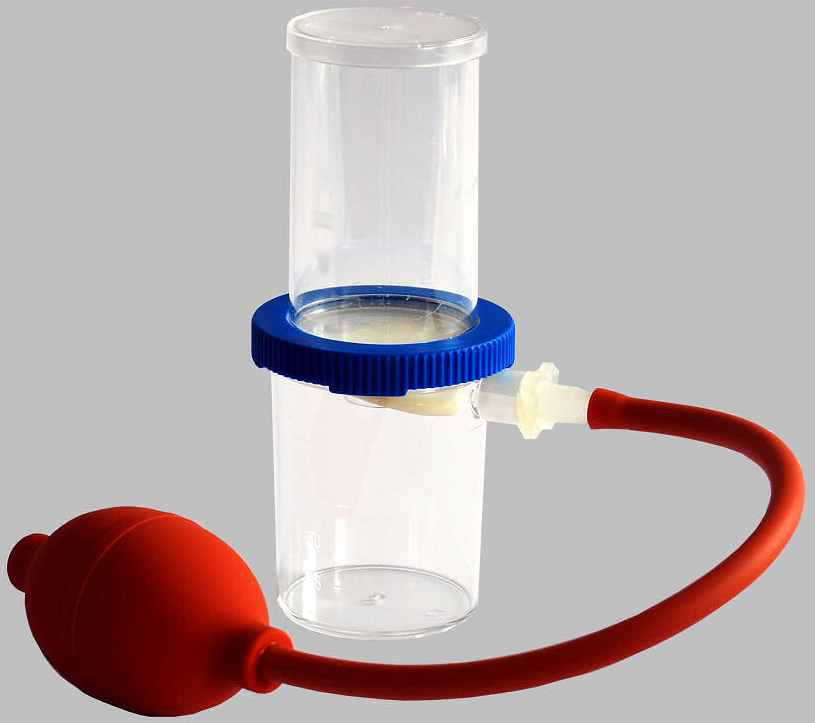
\includegraphics[width=10cm]{content/bilder/herzmodell.png}
    \caption{Aufbau des verwendeten Herzmodells \cite{Herz}.}
    \label{fig:Herz}
\end{figure}
